\documentclass[a4paper,12pt]{article}
% Package to make citations superscrit with brackets
\usepackage[super,square]{natbib}
% Package to change margin size
\usepackage{anysize}
\marginsize{2cm}{2cm}{1cm}{2cm}
% Package to make headers
\usepackage{fancyhdr}
\renewcommand{\headrulewidth}{0pt}
% Package for highligths (also strikethrough text)
\usepackage{soul}
% Colors for the references links
\usepackage[dvipsnames]{xcolor}
% Package to link references
\usepackage{hyperref}
\usepackage{amsmath}
\hypersetup{
    colorlinks=true,
    linkcolor=black,
    citecolor=CadetBlue,
    filecolor=CadetBlue,      
    urlcolor=CadetBlue,
}
% Package for lorem ipsum
\usepackage{lipsum}
% Package for multicolumn
\usepackage{multicol}
% Package for removing paragraph identations
\usepackage{parskip}
\setlength\columnsep{18pt}
% Sets bastract
\renewenvironment{abstract}
 {\par\noindent\textbf{\abstractname}\ \ignorespaces \\}
 {\par\noindent\medskip}

\usepackage{xcolor} 
\definecolor{verd}{rgb}{0.0, 1.0, 0.0} % positive
\definecolor{azul}{rgb}{0.0, 0.0, 1.0} % attention
\definecolor{rojo}{rgb}{1.0, 0.0, 0.0} % negative
\newcommand{\rojo}[1]{\textcolor{rojo}{#1}} 
\newcommand{\verd}[1]{\textcolor{verd}{#1}} 
\newcommand{\azul}[1]{\textcolor{azul}{#1}} 
% ------------------------------------------------------------ BEGIN DOCUMENT !
\begin{document}
% Makes header
\pagestyle{fancy}
\thispagestyle{empty}
\fancyhead[R]{\textit{Alejandro S. Vega-Nogales}}
\fancyhead[L]{Report Date: April 2025}
% Makes footnotes with an asterisk
\renewcommand*{\thefootnote}{\fnsymbol{footnote}}
\begin{center}
\Large{\textbf{Remote Sensing Assessment and Monitoring of Distributed Rooftop Solar Panel Arrays}}
\vspace{0.5cm}
{\color{gray}\hrule}
\medskip
\large\textbf{A report on methods for Computer Vision extraction and Photovoltaic energy forecasting} \\
\bigskip
\normalsize Alejandro S. Vega-Nogales, Data Scientist @ Maxar, CCOM MS Student \\
\vspace{0.1cm}
SIN: 801-13-7956 \quad github: \href{https://github.com/avega17}{avega17}  \quad email: \alejandro.vega1[at]upr.edu \\
\vspace{0.1cm}
\textit{UPRRP - Computer Science Department} \\
\vspace{0.1cm}
CCOM 6050: Final Project -- Midterm Project Report
\medskip
\normalsize
\end{center}
{\color{gray}\hrule} 
\vspace{0.4cm} 

\tableofcontents
\hfill
\clearpage

% Define path prefixes
\newcommand{\reportpath}{./report/src}

\section{Introduction}



\subsection{General Objective}
    \vspace{0.5cm}
    
    \textbf{Regional-scale surveys} of distributed \textit{rooftop PV solar panels}, and \textbf{site-level, short-term forecasting} of \textit{solar irradiance} used to estimate local PV power generation. \\
    \\
    This assessment will primarily produce counts of installed systems, estimates of surface area, estimated PV generation potential while monitoring will provide forecasts of local solar irradiance which are used to model estimates of PV energy generation at specific sites. \\
    \\ 
    The work developed for this thesis proposal is particularly inspired by and seeks to build upon the work realized, methodologies outlined, research gaps identified, and future work outlined in \cite{robinson_ms_planet_global_renewables_watch_2025}, \cite{Boussif_neurips_day_ahead_solar_forecasting_2023}, \cite{Li_solarcube_solar_forecasting_2024}, \cite{maxar_germany_pv_dataset}, \cite{Hu_solar_array_pitfalls_2022}, \cite{de-Hoog_sota_survey_2020}, \cite{Bansal_ssl_nowcasting_2022}, \cite{Jiang_rooftop_pv_assessment_2022}, \cite{Tremenbert_Kasmi_pyPV_roof_2023}, and \cite{Yu_deep_solar_2018}.

\subsection{Problem Statement and Motivation} 
% Brief description of the problem, objectives, methodology, and main findings. Less than 500 words.
% emphasize the distinction between energy source replacement and badly labeled "energy transition" which has never ocurred historically and instead new energy sources have always been added to the energy mix
The global response to climate change requires our civilization to implement a rapid transition to renewable energy sources in an effort to 
decarbonize the energy sector as much as possible. The fastest growing renewable energy source is by far \textit{photovoltaic} (PV) solar energy [cite]. Growing at over 41\% per year on average since 2009\cite{kruitwagen_global_inventory_pv_units_2021},
PV solar energy has far outpaced other renewable energy sources such as concentrated solar power (CSP), hydroelectric storage, geothermal energy, and, to a lesser extent, wind energy. 
% include figure for rapidly decreasing cost of PV energy and related battery storage technologies
This rapid growth has led to significant progress in international development goals such as the United Nations Sustainable Development Goals (SDG) which, among other things, 
addresses the population level needs for clean and affordable energy, and actions to tackle climate change and its impacts\cite{maxar_germany_pv_dataset}. 

Historically, one of the most effective means to ensure global cooperation and uniform implementation of environmental and energy policies has been through the establishment of multi-lateral 
international agreements such as the Montreal Protocol, the Kyoto Protocol, and, most recently, the Paris Climate Accords signed by (add figure of \% of countries signed and ref) countries. 
This agreement resulted in \textit{non-binding} commitments to reduce greenhouse gas emissions and goals to limit global warming to 1.5 - 2.0 degrees Celsius above pre-industrial levels. 
Notably, 87\% of these Nationally Determined Contributions (NDCs) aim to increase the share of renewable energy in their energy mix with half specifying empirical generation figures\cite{robinson_ms_planet_global_renewables_watch_2025}. 
\textbf{To maintain any semblance of international accountability to these commitments, these NDCs require extensive and accurate global monitoring and validation of any expansion of renewable energy infrastructure.}

To address this \textit{international policy problem} there has been a variety of efforts to assess the progress of each renewable energy source leading to recurring reports, inventories, assessments, and databases at the global, 
regional, and national levels. Many of these efforts prove insufficient due to only providing aggregated summaries or statistical extrapolations at the national level (IRENA, IEA, BP), or being limited to specific regions 
(i.e. primarily Europe, North America, and China). Particularly in the case of PV solar energy, there has been very significant progress over the last decade in the development of remote sensing and deep learning methods to assess 
the distribution of PV solar energy at the site, regional, and global levels (cite the many PV assessment papers).
Most recently, a collaboration between Microsoft, the Nature Conservancy, and Planet Labs\cite{robinson_ms_planet_global_renewables_watch_2025} has produced \textit{``Global Renewables Watch''}, 
a public dataset of industrial, commercial, and utility-scale PV solar energy and wind energy installations firmly establishing the \textbf{feasibility of using high-resolution satellite imagery and deep learning methods 
to assess the distribution of renewable energy infrastructure at the Planetary scale}.

These publications and datasets have primarily focused on large-scale, utility-scale PV solar energy installations (i.e. badly labeled ``solar farms'') which are 
typically located in remote areas with broad land availability and low land use conflicts. However, for some countries, land comes at a premium and concentrated large-scale solar energy installations are 
either not economically or politically feasible due to not being the most efficient use of land and other land use conflicts. This leads to countries where distributed, small-scale rooftop or building-integrated 
PV solar energy installations make up a significant portion of the total installed capacity which is not captured in assessment limited to large-scale installations. 
For example, Robinson et al\cite{robinson_ms_planet_global_renewables_watch_2025} and Kruitwagen et al\cite{kruitwagen_global_inventory_pv_units_2021} use a $\ge$ 10KW 
Additionally, intermittent renewable energy sources bring about a second \textit{technical problem} that also calls for assessments and inventories at a smaller spatial \textbf{and} temporal scale.

The intermittency of renewable energy sources such as wind and solar energy means that energy grid operators require accurate short-term forecasts of energy generation to ensure that national electric grid 
supply and demand are balanced. PV solar energy is particularly sensitive to local weather conditions and received solar irradiance which can both be monitored using 
remote sensing methods and local weather stations. There has been recent work in the use of geostationary satellites with high temporal resolution to provide short-term forecasts of solar irradiance at the site level\cite{Bansal_ssl_nowcasting_2022}, 
the use of spectral reflectance features in Computer Vision (CV) models for PV solar array detection\cite{He_universal_pv_spectral_index_2024}, and advances in spatio-temporal data fusion methods to improve the temporal resolution of very-high-resolution (VHR) satellite imagery\cite{Tremenbert_Kasmi_pyPV_roof_2023}. 

This project looks to outline the work required to address these interconnected challenges by tackling two core subproblems leveraging remote sensing data and advances in deep learning methods:
    % \vfill\null
    % \columnbreak
\end{multicols}

\subsubsection{[CCOM6120] Subproblem 1:}
    \textbf{Detection and Segmentation of distributed rooftop PV Systems using Computer Vision baseline models} 
    % \vspace{0.1cm}
    The first fundamental challenge lies in the automated, accurate, and scalable identification and geometric characterization of distributed rooftop PV panels using very-high-resolution (VHR) multispectral satellite imagery. 
    Generating reliable, up-to-date inventories of these small, dispersed assets is crucial for granular PV potential assessments\cite{Pueblas_workflow_rooftop_PV_assessment_sat_img_2023}\cite{Jiang_rooftop_pv_assessment_2022}, infrastructure planning, 
    monitoring deployment rates against policy goals\cite{de-Hoog_sota_survey_2020}, and producing the georeferenced geometry data required for accurate site-level solar irradiance forecasting and PV energy generation estimates\cite{Bansal_ssl_nowcasting_2022}.
    % \vfill\null
    % \columnbreak
    We will use the final project for CCOM6120 as preliminary work on this subproblem. We will explore baseline segmentation model architectures (e.g. UNet, FPN, PAN, SegFormer, etc.) and 
    encoder combinations (e.g. ResNet, EfficientNet, ViT, Swin, etc.) and how they perform on some existing published datasets. As part of the project we will develop and establish some 
    baseline data processing pipelines, model training workflows, and evaluation metrics. 

\subsubsection{[CCOM6050] Subproblem 2:} 
    \textbf{Hierarchical Spatial Clustering of global PV installations to optimize dataset generation} 
    Given a large, globally distributed set of Points-of-Interest (PoIs) representing Photovoltaic (PV) solar panel installations (potentially hundreds of thousands to millions), 
    the objective is to efficiently identify and retrieve subsets of relevant satellite imagery (rasters) from open access archives (e.g., STAC catalogs) that maximize the spatial and temporal coverage of the PoIs. 
    Our \textit{Optimization Goal} is to design an algorithmic framework that \textbf{maximizes} the spatial and temporal coverage of the PoIs by the fetched rasters while simultaneously 
    \textbf{minimizing} the number of raster queries and the volume of data downloaded and processed for model training. 

    \textbf{Why it's a problem:} 
    \begin{itemize}
        \item Naive querying strategies (i.e. per POI, or per cluster of POIs) quickly becomes very inefficient for large, globally distributed datasets of PoIs: 
        leads to excessive API calls or HTTP requests, redundant data retrieval, and high processing overhead.
        \item PV installations are naturally spatially clustered: \textit{but} these clusters are not known a priori and can span across arbitrary administrative boundaries or diverse geographic contexts.
        \item The spatial and temporal coverage of the PoIs is not uniform: being able to \textit{dynamically adjust} the size and shape of the query bounding boxes based on the density of PoIs in a 
        given area and the extent of specific raster items is crucial for efficient data retrieval.
    \end{itemize}

    We will use the final project for CCOM6050 as preliminary work on this subproblem. We will explore the use of data fusion with geospatial context from Overture Maps, the effectiveness of aggregating our hundreds of thousands of PoIs 
    using Discrete Global Grid Systems (DGGS) such as Uber's H3, and how we can leverage hierarchical spatial clustering algorithms over our H3 hexagon cells to produce a data structure that can be used to efficiently query and retrieve
    satellite imagery from open access catalogs.  

\subsubsection{[Future Thesis Work] Subproblem 3:} 
    \textbf{Solar irradiance forecasting at specific sites} 
    % \vspace{0.5cm}

    The second major challenge is analyzing \st{high-temporal-resolution surface reflectance} (intra-hour) time series of geostationary satellite imagery to produce accurate short-term forecasts of solar irradiance at specific sites. 
    This is a critical requirement for energy grid operators to ensure that supply and demand are balanced, especially in the case of intermittent renewable energy sources such as wind and solar energy. 

    
% \subsection{Specific Objectives}
%     \begin{enumerate}
%         \item Survey of rooftop Solar Panel \textit{Arrays} via Small Object Detection and Instance Segmentation using \href{https://www.maxar.com/maxar-intelligence/constellation}{very-high-spatial-resolution} (VHR) Multispectral \textit{satellite} imagery (MSI) ($\leq1$ meter/pixel) of installation locations sourced from a \textbf{global inventory of labeled PV arrays} collated from multiple scientific dataset publications [add citations] 
%         \item Leverage algorithms that can aid in optimizing our fetching of global satellite imagery from Open Access catalogs, and the use of \textbf{multi-spectral} data to improve the detection of PV arrays.
%         \item \textit{Near-term site-level forecasting} of solar \textbf{Global Horizontal  Irradiance} used to estimate PV power generation via data fusion with Spatio-temporal context from:
%         \begin{itemize}
%             \item Time-series frames from geostationary satellite sensors with high temporal resolution coarse spatial resolution
%             \item Historical Solar irradiance (e.g. NREL's National Solar Radiation Database)
%             \item Any available PV power generation ground-truth time series
%         \end{itemize}
        
%     \end{enumerate}
    
\subsection{Research Gaps and Contribution Goals}
    \begin{enumerate}
        \item Measure performance impact of SOTA Computer Vision architectures (e.g. ViT, Swin, CNN-Transformer hybrids) currently lacking in most recent publications and compare to established baselines (e.g. UNet, FPN, PAN, etc.)
        \item Regional, and global surveys are limited to large-scale farms using medium resolution sensors ($\sim10m$/pixel). On the other hand, studies using VHR aerial imagery usually only have coverage for local, city-scale surveys.
        We will use \textit{global 30cm yearly basemaps} or open access catalogs from VHR MSI sensors, primarily from Maxar, to perform a global survey of PV installations that includes both large-scale farms and distributed rooftop PV systems.
        \item Almost all notable studies (with the exception of \[cite GloSoFarID\]) exclusively use RGB image bands. Measure impact of use of PV-specific spectral indices\cite{He_universal_pv_spectral_index_2024} and specifically the benefits of including NIR + SWIR bands available in Maxar sensors
        \item Develop a solution that consciously tackles the challenges identified in \cite{Hu_solar_array_pitfalls_2022} for evaluating and performing comparisons of different remote sensing solar array assessment methodologies
        (distribution drift, test data quality, level of spatial-aggregation, and proprietary data)
    \end{enumerate}
    \hfill
% \lipsum[1]
{\color{gray}\hrule}
\clearpage
\section{Background}

\begin{multicols}{2}

\subsubsection{Earth Observation and Remote Sensing}

Remote sensing (RS) refers to the process of acquiring images and data of the planet’s surface using a variety of remote sensors in satellite and aerial vehicles (add citations from my prev paper). 
These sensors analyze electromagnetic radiation reflected or emitted from objects on the Earth’s surface, which is then processed to extract information about the objects and their properties. 
Besides traditional electro-optical (ie panchromatic and 3-channel RGB images (cite)) modern RS employs a variety of sensors and modalities such as multispectral 
(four or more non-overlapping bands in the electromagnetic spectrum), hyperspectral (more than 100 narrow bands), and even active sensors such as microwave altimeters or Synthetic
Aperture Radar (SAR) that emit their own radiation and measure the reflected signal to ”see” at night and through atmospheric obstructions like clouds and fog (cite myself or refs from prev paper). 
Analysis of source data from these remote sensors must handle a variety of nuanced characteristics of each sensor and the produced data. For our purposes and the scope of this report, we will limit our discussion
to the following characteristics: 

\begin{itemize}
    \item Spatial resolution: The level of detail in an image, typically measured in meters per pixel.
    \item Spectral resolution: The ability of a sensor to distinguish between different wavelengths of light.
    \item Temporal resolution: The frequency at which a sensor captures data over the same location.
    \item Radiometric resolution: The sensitivity of a sensor to detect variations in intensity, often represented by bit depth.
    \item Earth Observation (EO) data types:
        \begin{enumerate}
            \item Raster data: Gridded data representing continuous surfaces.
            \item Vector data: Discrete data represented as points, lines, or polygons.
            \item Time series data: Sequential data capturing changes over time over a specific area.
            \item Geospatial data cubes: Multidimensional arrays combining spatial, temporal, and spectral dimensions.
        \end{enumerate}
\end{itemize}

In the context of data engineering, geospatial data brings several optimization and operations that can ease the process of analyzing large volumes of this type of data.
One of the most relevant concepts for our project is a spatial index 
% A fundamental challenge in RS is the tradeoff that an individual sensor's orbit and design must make between spatial, spectral, and temporal resolution. 


\subsubsection{Computer Vision}

Computer Vision (CV) is a subfield of Artificial Intelligence and a discipline that deals with the problem of interpreting and extracting meaningful information from images (cite myself or refs from prev paper) 
in a manner similar to human vision. This field has seen significant advancements in recent years, particularly with the rise of deep learning methods and the spread of large, labeled datasets for many applications. 
RS and EO has seen an explosion of interest, publications, and datasets for DL methods since 2015 (cite EO paper from cloud computing course). Relevant CV tasks for our purposes include:

\begin{enumerate}
    \item Scene Classification: Assigning a label to an entire image based on its content (e.g., classifying an image as containing a PV array, rooftop, or vegetation).
    \item Object Detection: Identifying and localizing specific object classes (e.g., PV panels) within an image with (georeferenced) bounding boxes.
    \item Semantic Segmentation: Classifying each pixel in an image into predefined categories (e.g., PV panel array, rooftop, vegetation, background).
    \item Instance Segmentation: Similar to semantic segmentation, but differentiates between \textit{individual} instances (e.g., distinguishing between different PV panel arrays). 
\end{enumerate}

Some relevant CV architectures include Convolutional Neural Networks (CNNs), Vision Transformers (ViTs), Generative Adversarial Networks (GANs), and CNN-Transformer hybrids. 

% - Importance of satellite imagery for monitoring renewable energy infrastructure.
% - Characteristics of PV arrays as seen from space (spectral, spatial).
% - Brief overview of relevant sensor types (multispectral, VHR).

\subsection{SpatioTemporal Asset Catalogs}
\label{subsec:stac} % Added label for cross-referencing

A SpatioTemporal Asset Catalog (STAC) is a specification schema that provides a standardized, open, and interoperable way to describe and catalog geospatial information. 
It enables \textbf{efficient searching, discovery, and access} to imagery, sensor data, and other Earth observation (EO) products. 
STAC has emerged as a crucial component in modern geospatial data infrastructure and workflows, addressing the challenges of 
managing and accessing vast volumes of EO data when performing large-scale analysis.

Key features and benefits of STAC include:
\begin{itemize}
    \item \textbf{Standardization}: STAC defines a common language for describing geospatial assets, using JSON to structure metadata. 
    This includes spatial extent (geometry), temporal coverage (datetime), data providers, licensing, and links to the actual data files (assets) and related resources. 
    \item \textbf{Discoverability}: The STAC metadata structure enables powerful search capabilities. 
    Users can query catalogs based on spatial (e.g. single point, or Polygon features) and temporal criteria, as well as other metadata fields like cloud\_cover, making it easier to find relevant data across diverse collections and providers without needing to understand provider-specific APIs.
    \item \textbf{Accessibility}: STAC catalogs typically link directly to the underlying data assets, often hosted in cloud object storage (e.g. AWS S3, Google Cloud Storage). 
    This allows for direct access to data, often in cloud-optimized formats like Cloud-Optimized GeoTIFF (COG), 
    enabling users to stream or process data without downloading entire image strips.
    \item \textbf{Interoperability}: The specification is designed to be extensible, allowing communities to add specific metadata fields relevant to their domain 
    while maintaining core compatibility. This has led to fast and widespread adoption and the development of a rich ecosystem of tools and services that support STAC. 
    \item \textbf{Cloud-Native Focus}: STAC is inherently cloud-native. It facilitates the creation of large-scale, dynamic catalogs of EO data that can be easily accessed and processed in the cloud, reducing data duplication and transfer costs.
\end{itemize}

The STAC specification consists of several core components:
\begin{itemize}
    \item \textbf{Item}: The fundamental unit in STAC, representing a single spatiotemporal asset (e.g., a satellite scene) described by its metadata and links to data files.
    \item \textbf{Collection}: A group of related STAC Items that share common metadata, such as sensor type, processing level, or geographic region.
    \item \textbf{Catalog}: A flexible structure that organizes STAC Collections and Items, often hierarchically, to facilitate browsing and discovery. Catalogs can link to other Catalogs, Collections, or Items.
    \item \textbf{API}: STAC also defines an API specification (STAC API) that provides a \textit{standardized} way to query and serve STAC metadata \textit{over the web}. This allows for dynamic searching and filtering of large catalogs.
\end{itemize}

The shift towards STAC represents a paradigm change from traditional data download workflows to more dynamic, query-driven access. 
Instead of downloading large, monolithic datasets, users can precisely identify and access only the data they need, often processing it in place and at scale in the cloud.
This approach is critical for handling the ever-increasing volume of EO data (hundreds of TB's daily!) and enabling scalable, on-demand geospatial analysis. 
The STAC ecosystem includes a variety of open-source tools that lower the barrier to adoption, such as \texttt{pystac} (Python library for creating and manipulating STAC objects), 
\href{https://radiantearth.github.io/stac-browser/#/external/maxar-opendata.s3.amazonaws.com/events/catalog.json?.language=en}{STAC Browser} (web-based exploration of STAC catalogs), 
and clients for various programming languages.


\subsection{Discrete Global Grid Systems}
% * Introduction to DGGS concepts.
% * Specifics of H3: hexagonal, hierarchical, indexing capabilities (`h3.geo_to_h3`, `h3.k_ring`, `h3.grid_distance`).
% * Rationale for using H3 as the foundational grid for spatial aggregation and analysis (Li et al., 2024, for grid-based significance thinking; 
% Oje et al., 2025, for context on DGGS performance, even if HierGP is adaptive).

\subsection{Minimum Spanning Trees for Spatial and Hierarchical Clustering}
% * Concept of MSTs in graph theory.
% * Application of MSTs in clustering: identifying natural groupings by cutting edges.
% * Advantages for spatial data: ability to find clusters of arbitrary shapes (Gagolewski et al., 2023).

\subsection{Research Gaps and Contribution Goals}
    \begin{enumerate}
        \item Measure performance impact of SOTA Computer Vision architectures (e.g. ViT, Swin, CNN-Transformer hybrids) currently lacking in most recent publications and compare to established segmentation baselines (e.g. UNet, FPN, PAN, etc.)
        \item Regional, and global surveys are limited to large-scale farms using medium resolution sensors ($\sim10m$/pixel). On the other hand, studies using VHR aerial imagery usually only have coverage for local, city-scale surveys.
        We will use \textit{global 30cm yearly basemaps} or open access catalogs from VHR MSI sensors, primarily from Maxar, to perform a global survey of PV installations that includes both large-scale farms and distributed rooftop PV systems.
        \item Almost all notable studies (with the exception of (cite GloSoFarID)) exclusively use RGB image bands. Measure impact of use of PV-specific spectral indices\cite{He_universal_pv_spectral_index_2024} and specifically the benefits of including NIR + SWIR bands available in Maxar sensors
        \item Develop a solution that consciously tackles the challenges identified in \cite{Hu_solar_array_pitfalls_2022} for evaluating and performing comparisons of different remote sensing solar array assessment methodologies
        (distribution drift, test data quality, level of spatial-aggregation, and proprietary data)
    \end{enumerate}


\end{multicols}


% \subsubsection{Data Fusion}

% \begin{enumerate}
%     \item Definition: combining data from multiple sources to achieve improved information quality or inference compared to using sources individually\cite{Castanedo_trad_data_fusion_2013} 
%     \item (Geospatial) Coherence\cite{Ghamisi_Multisource_and_Multitemporal_Data_Fusion_in_Remote_Sensing_2019}
%     \item Remote Sensing Fusion types\cite{Ghamisi_Multisource_and_Multitemporal_Data_Fusion_in_Remote_Sensing_2019}\cite{Li_DL_multimodal_RS_data_fusion_review_2022}
%     \begin{itemize}
%         \item Spatio-Spectral Fusion: Enhancing spectral resolution using spatial information (e.g., Pansharpening) or vice versa.\cite{Ghamisi_Multisource_and_Multitemporal_Data_Fusion_in_Remote_Sensing_2019}\cite{Zhang_panchromatic_and_msi_fusion_for_RS_and_EO_2023}
%         \item Spatio-Temporal Fusion: Combining high spatial resolution/low temporal frequency data with low spatial resolution/high temporal frequency data to generate a fused dataset with 
%         high resolution in both domains.\cite{Ghamisi_Multisource_and_Multitemporal_Data_Fusion_in_Remote_Sensing_2019} \textbf{This is the core fusion type for the second subproblem of this project}. 
%     \end{itemize}
%     \item Data Fusion Abstraction Levels\cite{Hussain_DL_Data_Fusion_review_2024}
%     \begin{itemize}
%         \item Early fusion (pixel/signal level): Combining raw sensor data directly 
%         \item Intermediate fusion (feature level): Extracting relevant features from each sensor first and then combining them
%         \item Late fusion (symbol/decision level): Each source produces an independent decision, which is then combined to produce a final output
%         % \item Hybrid fusion (combination of levels)
%     \end{itemize}
%     \item  A review from Castanedo\cite{Castanedo_trad_data_fusion_2013} also categorizes fusion based on the relationship between data sources (complementary, redundant, cooperative)
%     \item The rise of Deep Learning (DL) has significantly impacted the field, with reviews listing CNNs, LSTMs, GANs, and Transformers as the most relevant architectures for data fusion\cite{Li_DL_multimodal_RS_data_fusion_review_2022}\cite{Hussain_DL_Data_Fusion_review_2024}.
% \end{enumerate}


{\color{gray}\hrule}
\medskip
{\color{gray}\hrule}
\begin{center}
\section{Methodology}
% \textbf{Here you will describe your:}
% \begin{itemize}
%     \item Experiments done and pending
%     \item Tools, software, code 
%     \item Data available (Description, source)
%     \item Results (if any)    
% \end{itemize} 
% Create a subsection for each part described in the methodology. These subsections can be modified based on the work or progress made during the current month. Additionally, you may create separate sections if needed, for example, to distinguish results based on different strategies. This template is flexible and can be adapted for better presentation.

\bigskip
\end{center}
{\color{gray}\hrule}

\subsection{Datasets}
\subsubsection{RS imagery and locations of PV arrays}
    Datasets in bold were used in the data preparation and analysis described in the next section. 
    \begin{table*}[htbp]
        \centering
        \scriptsize
        \caption{Summary of identified datasets for PV array segmentation and detection.}
        \begin{tabularx}{.95\textwidth}{|p{0.5\textwidth}|p{0.1\textwidth}|p{0.1\textwidth}|p{0.15\textwidth}|}  \hline
            \textbf{Dataset Title} & \textbf{Author, Year} & \textbf{DOI Links} & \textbf{Label Information} \\
                \hline
                A 10-m national-scale map of ground-mounted photovoltaic power stations in China of 2020 & Feng et al., 2024 & \href{https://doi.org/10.1038/s41597-024-02994-x}{Paper}\linebreak \href{https://doi.org/10.57760/sciencedb.o00121.00001}{Dataset} & 5K Positive samples and 5K negative samples in China, spring 2020 \\
                \hline
                GloSoFarID: Global multispectral dataset for Solar Farm ID & Yang, 2024 & \href{https://doi.org/10.48550/arXiv.2404.05180}{Paper}\linebreak \href{https://github.com/yzyly1992/GloSoFarID/tree/main/data_coordinates}{Dataset} & 6,793 PV samples across 3 years \\
                \hline
                Vectorized solar PV installation dataset across China & Liu et al., 2024 & \href{https://doi.org/10.1038/s41597-024-04356-z}{Paper}\linebreak \href{https://github.com/qingfengxitu/ChinaPV}{Dataset} & 3,356 PV labels \\
                \hline
                \textbf{A solar panel dataset of very high resolution satellite imagery} & Clark et al., 2023 & \href{https://doi.org/10.1038/s41597-023-02539-8}{Paper}\linebreak \href{https://doi.org/10.6084/m9.figshare.22081091.v3}{Dataset} & 2,542 object labels \\
                \hline
                Crowdsourced aerial images with annotated solar PV arrays & Kasmi, 2023 & \href{https://doi.org/10.1038/s41597-023-01951-4}{Paper}\linebreak \href{https://doi.org/10.5281/zenodo.6865878}{Dataset} & $>$28K PV points\linebreak 13K$+$ segmentation masks \\
                \hline
                Georectified polygon database of ground-mounted large-scale solar PV sites in US & Sydny, 2023 & \href{https://doi.org/10.1038/s41597-023-02644-8}{Paper}\linebreak \href{https://www.sciencebase.gov/catalog/item/6671c479d34e84915adb7536}{Dataset} & 4,186 data points \\
                \hline
                \textbf{An Artificial Intelligence Dataset for Solar Energy Locations in India} & Ortiz, 2022 & \href{https://doi.org/10.1038/s41597-022-01499-9}{Paper}\linebreak \href{https://github.com/microsoft/solar-farms-mapping/blob/main/data/solar_farms_india_2021_merged_simplified.geojson}{Dataset} & 117 geo-referenced solar installations \\
                \hline
                \textbf{A global inventory of photovoltaic solar energy generating units} & Kruitwagen et al., 2021 & \href{https://doi.org/10.1038/s41586-021-03957-7}{Paper}\linebreak \href{https://doi.org/10.5281/zenodo.5005867}{Dataset} & 50,426 training samples\linebreak 68,661 predicted labels \\
                \hline
                Multi-resolution dataset for PV panel segmentation & Jiang, 2021 & \href{https://doi.org/10.5194/essd-13-5389-2021}{Paper}\linebreak \href{https://doi.org/10.5281/zenodo.5171712}{Dataset} & 3,716 PV data points \\
                \hline
                \textbf{A harmonised, high-coverage, open dataset of solar PV installations in the UK} & Stowell et al., 2020 & \href{https://doi.org/10.1038/s41597-020-00739-0}{Paper}\linebreak \href{https://zenodo.org/records/4059881}{Dataset} & 265,418 data points \\
                \hline
                \textbf{Harmonised global datasets of wind and solar farm locations and power} & Dunnett et al., 2020 & \href{https://doi.org/10.1038/s41597-020-0469-8}{Paper}\linebreak \href{https://doi.org/10.6084/m9.figshare.11310269.v6}{Dataset} & 35,272 PV installations \\
                \hline
                \textbf{Distributed solar photovoltaic array location and extent dataset} & Bradbury, 2016 & \href{https://doi.org/10.1038/sdata.2016.106}{Paper}\linebreak \href{https://doi.org/10.6084/m9.figshare.3385780.v4}{Dataset} & 19,433 PV modules in 4 California cities \\
                \hline
        \end{tabularx}
        \label{tab:pv_datasets}
    \end{table*}

\begin{multicols}{2}

\subsection{Python Libraries and other computational tools}
\begin{itemize}
    \item \textit{Python 3.10} - programming language  
    \item \textit{PyTorch 2.0} - deep learning framework 
    \item \textit{jupyterlab} - web-based interactive development environment for Jupyter notebooks
    \item \textit{numpy + xarray} - array processing
    \item \textit{Geopandas} - Geospatial data manipulation and analysis
    \item \textit{duckdb} - an in-process SQL OLAP database management system
    \item \textit{cubo} - a library for working with cuboids (3D arrays) in Python
    \item \textit{stac-geoparquet} - Convert STAC items between JSON, GeoParquet, pgstac, and Delta Lake; allows users to access a large number of STAC items in bulk without making repeated HTTP requests
    \item \textit{openeo} - python client for the OpenEO API
    \item \textit{Rasterio} - Raster data reading and writing
    \item \textit{GDAL} - Geospatial data abstraction library
    \item \textit{mamba} - a faster alternative to the conda package manager
    \item \textit{rastervision} - a framework for computer vision and deep learning in remote sensing
    \item \textit{PyTorch Lightning} - a lightweight wrapper for PyTorch to accelerate model training and testing
    \item \textit{TorchGeo} - a library for deep learning on geospatial data which includes datasets and pretrained models
    \item \textit{segmentation-models-pytorch} - a library for pre-trained semantic segmentation models and vision encoders in PyTorch
    % \item \textit{super-gradients} - a library for transfer learning and training of SOTA CV models
    % \item \textit{data-gradients} - a library designed for computer vision dataset analysis and visualization
    \item \textit{torchmetrics} - a library for computing model evaluation metrics in PyTorch
\end{itemize}

\subsubsection{Hardware and Compute Resources}

\begin{itemize}
    \item Personal Developer Machine: 16'' Macbook Pro 2021, M1 Max, 32GB RAM, PyTorch supported mps accelerator
    \item Google Colab Pro+: \$50/month subscription used to efficiently train models on cloud GPUs (up to Nvidia A100) and test clustering algorithms on GPU
    \item Google Earth Engine [Future]: cloud-based geospatial analysis platform for large-scale remote sensing data processing 
    \item Microsoft Planetary Computer [Future]: cloud-based geospatial analysis platform for large-scale remote sensing data processing
    \item AWS [Future]: hosts many open-access geospatial datasets including STAC Catalogs and offers cheap cloud object storage
    
\end{itemize}

\subsubsection{Code Repository}

As of writing, the \href{https://github.com/avega17/CCOM_MS_Spring_2025_EO_PV_research}{Github repo} where this report and associated code is hosted is public.

% \subsection{Evaluation}
    % \begin{itemize}
    %     \item Goal(s): Assess accuracy of reconstructed time series 
    %     \item Metrics (including their normalized versions):
    %     \begin{itemize}
    %         \item RMSE (Root Mean Square Error)
    %         \item MAE (Mean Absolute Error)
    %         \item MAPE (Mean Absolute Percentage Error)
    %         \item MBD (Mean Bias Deviation)
    %         \item R2 (Coefficient of Determination)
    %         \item PSNR (Peak Signal-to-Noise Ratio)
    %         % validate which are useful for STF and regression tasks
    %     \end{itemize}
    %     \item Baseline(s):
    %         \begin{itemize}
    %             \item Persistence model 
    %             \item Clear sky components
    %         \end{itemize}
    % \end{itemize}
    % \subsubsection{Computer Vision Models}
    %     \begin{itemize}
    %         \item Dice Loss
    %         \item mean Intersection over Union (mIoU): 
    %     \end{itemize}

% \subsection{Expected Results}

% \begin{enumerate}
%     \item Subproblem 1: 
%         \begin{itemize}
%             \item Description of the expected results
%             \item Description of the expected results
%         \end{itemize}
%     \item Subproblem 2:
%         \begin{itemize}
%             \item Description of the expected results
%             \item Description of the expected results
%         \end{itemize}
%     \item Subproblem 3:
%         \begin{itemize}
%             \item Description of the expected results
%             \item Description of the expected results
%         \end{itemize}
% \end{enumerate}

\end{multicols}
\bigskip
{\color{gray}\hrule}
\begin{center}
\section{Spatial Hierarchical Clustering applied to DGGS: Algorithms and Complexity}
\textbf{Here we will go into detail on our algorithm design and approach for optimization of STAC queries when generating our dataset.}
\bigskip
\end{center}
{\color{gray}\hrule}

% \begin{multicols}{2}

\subsection{Data Ingestion and Pre-processing}
\label{subsec:data_ingestion}

\paragraph{Dataset Acquisition and Management} 
We download PV installation datasets from various academic repositories including Zenodo, figshare, GitHub, and ScienceBase. 
The datasets listed in the table below are publicly available and can be used for training and testing of computer vision models for PV array segmentation and detection. 
They were selected based on their availability, size, area coverage, and relevance to the problem of PV array segmentation and detection.
The data records are available in multiple vector file formats (GeoJSON, GeoPackage, Shapefile), which we standardize using our data pipeline. a
We utilize the \texttt{datahugger} library to fetch datasets from Zenodo and figshare, \texttt{sciencebasepy} for accessing the USGS ScienceBase Catalog, 
and custom functions for GitHub-hosted datasets. Dataset metadata is stored in a structured JSON configuration file to track sources, DOIs, and formats. 
For implementation details of this subsection, we refer the reader to the \href{https://github.com/avega17/CCOM_MS_Spring_2025_EO_PV_research/blob/main/fetch-pv-datasets-ESDA.ipynb}{fetch-pv-datasets-ESDA.ipynb} notebook.

\paragraph{Standardization to GeoParquet}
We convert all vector dataset files to GeoParquet format using \texttt{geopandas}. GeoParquet extends the Apache Parquet columnar storage format with geospatial capabilities, providing significant advantages:
\begin{itemize}
    \item \textit{Efficient storage} with built-in compression, reducing file sizes compared to GeoJSON and other spatial vector formats
    \item \textit{Columnar storage format} optimized for analytical queries and filtering operations
    \item \textit{Spatial indexing and predicate pushdown} capabilities for efficient geospatial operations over supported geometry types
    \item \textit{Wide ecosystem compatibility} with modern geospatial and cloud-optimized tools and workflows
\end{itemize}

This provides a space complexity reduction. For example, the cumulative size of the 5 datasets(cite) we worked with this semester was 690.5 MB in GeoJSON and GeoPackage formats, 
while after consolidation and conversion to GeoParquet the size was reduced to 107.3MB. This is largely due to the inherent compression capabilities of the Parquet format, from removing unused columns, 
and filtering out invalid geometries. 

\paragraph{Consolidation and Deduplication}
After standardizing individual datasets, we:
\begin{enumerate}
    \item Consolidate all datasets into a single DuckDB database with spatial extensions enabled
    \item Create a unified schema with standardized columns (geometry, area, source dataset, etc.)
    \item Perform spatial deduplication to remove overlapping polygons using spatial indices
    \item For CV models, filter to only retain valid polygon geometries (POLYGON, MULTI-POLYGON) for segmentation training
\end{enumerate}

The running time for the deduplication process is reduced by using spatial indices as for each record we only need to compare nearby geometries as established by the spatial index.


\paragraph{Geospatial Enrichment}
We enrich the consolidated PV dataset with administrative boundary information from the Overture Maps project:
\begin{enumerate}
    \item Spatial join with Overture divisions (countries, regions, counties)
    \item Administrative division matching (ISO country codes and region names, and division\_ids for future querying) for each PV installation
    \item Aggregation statistics at country and region levels
    \item Choropleth visualizations of PV distribution by country and region
    \item Leafmap interactive scatterplot map for visualizing PV installations coordinates in Jupyter notebooks
    \item Adding geographic context allows us to train by country or even regional models adapted to local conditions
    \item Enables efficient querying of PV installations by administrative divisions
\end{enumerate}

\paragraph{H3 Indexing and Spatial Aggregation}
To efficiently organize and query the global PV dataset, we utilize H3, the hierarchical hexagonal DGGS discussed above.
H3 provides a hierarchical structure of hexagonal grid cells, allowing for efficient spatial indexing and querying. There are \texttt{duckdb} and \texttt{python} bindings available for H3,
which we use to index the PV dataset and perform spatial operations.
\begin{enumerate}
    \item Each PV installation is assigned an H3 index at optimal resolution based on its size
    \item Common H3 resolution (level 5, $\sim$250km$^2$ hexagons) added for regional aggregation
    \item Efficient spatial clustering and adaptive subdivisions using H3 hierarchy
    \item Spatial joins with geospatial data layers (Overture Maps) using H3 indices as common keys
\end{enumerate}

\subsection{Graph Construction from H3 Grid Cells for MST [Future Work]}

A Mutual Reachibility Graph (MRG) is an undirected, weighted graph where each node represents a point in the dataset and edges represent the mutual reachability distance between points.
The foundation for our hierarchical spatial clustering is a graph $G=(V, E_w)$, where the set of vertices $V$ represents H3 grid cells containing PV installations, and $E_w$ is the set of weighted edges quantifying the proximity between these cells.

\paragraph{Node Definition}
Instead of the set of raw input data points, the geometric centroids of each unique H3 cell that contains one or more PV PoIs at a chosen analysis resolution (e.g., $res_A$) becomes a node $v \in V$. Let $N = |V|$ be the total number of such H3 cells.

\paragraph{Edge Weight Definition}
The primary metric for defining the weight (or "distance") between any two H3 cell nodes, say $c_a$ and $c_b$, is the H3 grid distance: $w(c_a, c_b) = \texttt{h3.grid\_distance}(c_a, c_b)$. 
This function returns the shortest number of steps (hops) on the H3 grid required to move from $c_a$ to $c_b$.
\begin{itemize}
    \item This topological (i.e. not geometric) distance inherently captures spatial adjacency and connectivity within the H3 grid structure. 
    The \texttt{h3.grid\_distance} function itself is efficient and can be considered $O(1)$ constant time for a single pair\cite{H3_Algorithm1}, typically operating in constant time or time proportional to the distance, as it relies on arithmetic and geometric operations on cell IDs.
    \item Using \texttt{h3.grid\_distance} directly as the edge weight prioritizes connecting H3 cells that are close in terms of grid topology for the MST.
\end{itemize}
% While this is the primary metric, future work could explore hybrid weighting schemes that incorporate feature similarity between H3 cells (e.g., similarity in PV density, installation dates, or STAC-derived land cover characteristics) in addition to the grid distance.

\paragraph{Graph Sparsification for Scalability}
A naive approach to constructing a complete graph with edges between all $N$ H3 cells would require computing $O(N^2)$ edge weights, making MST computation intractable for large $N$. Therefore, graph sparsification is essential:
\begin{enumerate}
    \item \textbf{$k$-Ring Neighbors:} For each H3 cell $c_i$, consider only edges to its immediate H3 neighbors within a small $k$-ring (e.g., using \texttt{h3.k\_ring(}$c_i$\texttt{, k\_val)} where $1 \geq k' \leq 3$). 
    This bounds the number of candidate edges to $O(N \cdot 7^{k'})$ where N is the number of H3 cells with PV installations and further bounded by only considering grid cells with PV installations.
    \item \textbf{Maximum H3 Distance Threshold:} Alternatively, consider edges only between H3 cells $c_a, c_b$ if $\texttt{h3.grid\_distance}(c_a, c_b) \leq D_{\max}$, where $D_{\max}$ is a predefined maximum H3 distance. 
    The number of edges here would depend on the spatial distribution of PV-containing H3 cells and $D_{\max}$.
\end{enumerate}
These sparsification strategies significantly reduce the number of edges ($E_{sparse}$) in the graph, typically to $O(N \cdot \text{avg\_degree})$, making subsequent MST algorithms (like Kruskal's or Prim's, which scale with the number of edges) computationally feasible. 
The choice of sparsification parameters ($k'$ or $D_{\max}$) involves a trade-off between computational cost and the fidelity of the resulting MST compared to one built on a complete graph.
The resulting sparse, weighted graph of H3 cells is the direct input to the MST construction algorithms. 

\subsection{MST Construction: Running Time and Parallel Optimizations [Future Work]}
% * Algorithm: Parallel GeoFilterKruskal (GFK) with MemoGFK optimization (Wang et al., 2021).
% * Justification: Scalability for large numbers of H3 cells, memory efficiency.
% * *(If HDBSCAN*-like density focus is explored: discuss core distance definition for H3 cells and Wang et al.'s specialized well-separation).*
\label{subsec:mst_construction}

Once the sparse graph of H3 cells $G=(V, E_{sparse})$ is constructed, the next crucial step is the construction of a MST. 
The MST will form the backbone for the subsequent hierarchical clustering and dendrogram generation as described in \cite{Wang_Yu_Gu_Shun_2021}. 
Therefore we need efficient algorithms for MST construction, especially given the potentially large number of H3 cells ($N$) involved in a global or regional analysis.

\paragraph{Classic MST Algorithms and Complexity}
Several classic algorithms are foundational for MST construction on a graph with $N$ vertices and $E_{sparse}$ edges:
\begin{itemize}
    \item \textbf{Kruskal's Algorithm:} Sorts all $E_{sparse}$ edges by weight and adds them if they connect two previously unconnected components. Complexity: $O(E_{sparse} \log E_{sparse})$ or $O(E_{sparse} \log N)$ using a Union-Find data structure.
    \item \textbf{Prim's Algorithm:} Grows the MST from a start vertex, iteratively adding the cheapest edge to an unvisited vertex. Complexity: $O(E_{sparse} \log N)$ with a binary heap, or $O(E_{sparse} + N \log N)$ with a Fibonacci heap.
    \item \textbf{Boruvka's Algorithm:} Iteratively adds the minimum weight edge incident to each component. Complexity: $O(E_{sparse} \log N)$, and is inherently parallelizable.
\end{itemize}
Given our graph sparsification, where $E_{sparse}$ is typically $O(N)$ (e.g., when using $k$-ring neighbors with small $k'$), these algorithms become significantly more tractable. For example, Kruskal's algorithm would have a complexity of roughly $O(N \log N)$.

\paragraph{Parallel Optimizations for EMST and Adaptations for H3 Graphs [Future Work]}
For Euclidean Minimum Spanning Trees (EMST) on point data, where the graph is implicitly dense, Wang et al. (2021) proposed parallel algorithms using Well-Separated Pair Decompositions (WSPDs) to reduce effective pairs to $O(N)$, and a parallel GeoFilterKruskal (GFK)\cite{Wang_Fast_Parallel_EMST_HDBSCAN_2021}. 
Their parallel EMST algorithm achieves $O(N^2)$ work in constant dimensions but, importantly, has a polylogarithmic depth, $O(\log^2 N)$, (i.e., the longest series of sequential operations in the parallel algorithm) enabling substantial parallel speedups. 

For our H3 graph, which is already sparse due to the strategies in Section \ref{subsec:graph_construction_h3}:
\begin{enumerate}
    \item Parallel versions of Kruskal's (like the author's Parallel GFK) or Boruvka's algorithm are directly applicable and offer good performance.
    \item The principle of Wang et al.'s GFK/MemoGFK (processing edges in batches based on weight ranges) can still be beneficial for managing memory and improving cache efficiency if $E_{sparse}$ remains very large (e.g., for global-scale analysis with a high average degree after sparsification).
\end{enumerate}
As the authors showed in their runtime decomposition figure, the MST Construction step has by far the shortest running time compared to their WSPD and Dendogram algorithms.
The effort in constructing the MST efficiently is well-justified as the relatively fast computation of MSTs, especially with parallel and memory optimizations on sparse graphs, makes this approach viable for large-scale, planetary datasets of H3 cells.

\subsection{Generating a Hierarchy of Clusters: Dendrogram Construction and H3 Multi-resolution}
\label{subsec:dendrogram_construction}

Following construction of the MST from H3 cells, the next step is to derive a hierarchy of clusters. 
This is achieved by generating a dendrogram, which visually and structurally represents the nested groupings of H3 cells based on their proximity or similarity as captured by the MST. 
The dendrogram is fundamental to hierarchical clustering, allowing for the exploration of cluster structures at various levels of granularity and informing our selection of STAC raster assets.

\paragraph{Dendrograms from MSTs}
A single-linkage dendrogram can be directly constructed from an MST. Conceptually, if MST edges are sorted by weight (e.g., \texttt{h3.grid\_distance}), the dendrogram represents 
the sequence of merges (in an agglomerative sense) or splits (in a divisive sense) of H3 cells. Each internal node in the dendrogram corresponds to an edge in the MST, and 
its height in the dendrogram is typically proportional to the weight of that edge. Cutting the dendrogram at a certain height yields a flat partitioning of the H3 cells into $k$ clusters.

\paragraph{Efficient Dendrogram Construction}
Traditionally, dendrograms are built sequentially, often using a Union-Find data structure, which for large $N$ (number of H3 cells) can be a bottleneck ($O(N \log N)$ but serial). 
For the scope of this project, we briefly highlight the development of parallel algorithms for Single-Linkage Dendrogram (SLD) computation that offer improved theoretical guarantees and practical speedups. 
For instance, algorithms by Dhulipala et al. (2024) achieve $O(N \log h)$ work (where $h$ is dendrogram height) with practical CPU implementations like RC-Tree Tracing (RCTT) \cite{dhulipala_Optimal_Parallel_Dendrogram_2024}. 
Furthermore, PANDORA (Sao et al., 2024) provides a work-optimal ($O(N \log N)$) GPU-accelerated approach robust to skewed dendrograms \cite{sao_PANDORA_GPU_Dendrogram_2024}. 
The use of such efficient methods is crucial for handling the scale of H3 cell datasets derived from global PV PoIs, ensuring the dendrogram generation step does not act as a bottleneck for the overall workflow 
as shown in Wang et al.'s runtime decomposition figure \cite{Wang_Fast_Parallel_EMST_HDBSCAN_2021} below.

\subsection{Optimized STAC Querying [Future Work]}

\paragraph{Integrating H3 Hierarchy for Optimized STAC Asset Selection and Coverage}
The primary focus is on leveraging the resulting hierarchy in conjunction with H3's hierarchical capabilities to efficiently generate the MST-based geometries used for querying STAC assets.
While the MST-derived dendrogram provides a \textit{data-driven hierarchy} of PV-containing H3 cells, Uber H3's native hierarchical functions are instrumental in \textbf{relating these clusters to STAC raster asset extents and administrative boundaries} (e.g., countries). 
This integration is key to optimizing the selection of STAC assets to maximize PV coverage while minimizing data redundancy for initial querying, and then enabling selective accumulation of imagery for analysis.

\begin{enumerate}
    \item \textbf{Representing STAC Raster Footprints with H3 and joining with PV H3 cells:}
        For each candidate STAC raster Item, its geographic footprint (a bounding box polygon) is converted into a set of H3 cells at a chosen base analysis resolution (e.g., $res_A$) using the \texttt{h3.polygon\_to\_cells(h3shape, res)} function. 
        This creates a \textit{discrete, gridded representation of each raster's coverage}.

    \item \textbf{Contextualizing Raster H3 Cells with AOI Geometries:}
        The H3 cells derived from STAC raster polyfills of H3 cells are then spatially intersected with the geometry of an Area-of-Interest (AOI) (from Overture Maps \textit{division\_area} theme) which we convert to H3 Cells using the same function. 
        This step identifies, for each AOI, the subset of H3 cells from each overlapping raster that falls within its boundaries. We specifically only track raster-derived H3 cells that also correspond to H3 cells containing our PV PoIs. 
        In this way we can capture only the "cells of Interest" (COIs) for each STAC raster item and AOI.
        
        \begin{figure}[ht]
            \centering
            \begin{subfigure}{\textwidth}
                \centering
                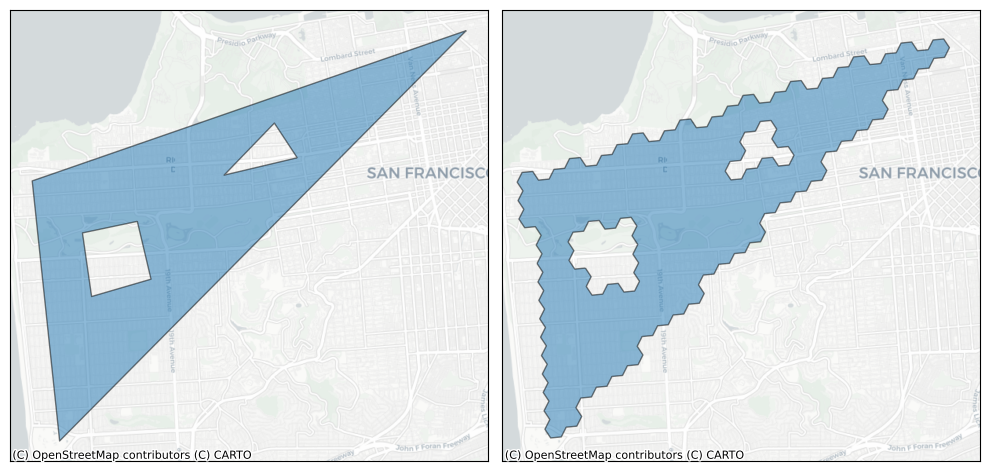
\includegraphics[width=0.6\textwidth]{report/assets/figures/h3_polygonToCells_example_res9.png}
                \caption{Polyfill of H3 cells at resolution 9 of an example Polygon}
            \end{subfigure}
            
            \begin{subfigure}{\textwidth}
                \centering
                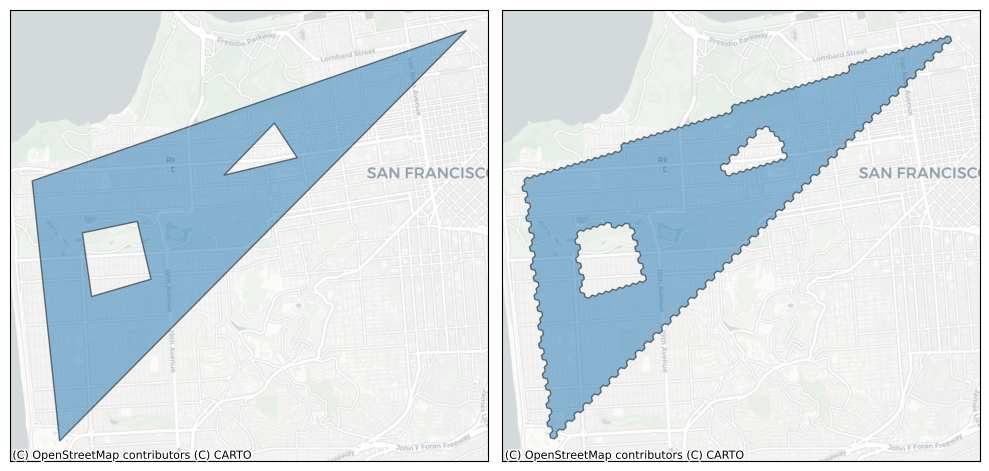
\includegraphics[width=0.6\textwidth]{report/assets/figures/h3_polygonToCells_example_res10.png}
                \caption{Polyfill of H3 cells at resolution 10 of the same example Polygon with higher precision}
            \end{subfigure}
            % \caption{Representation of a STAC item footprint at different H3 resolutions using \texttt{polygon\_to\_cells()}. Higher resolutions provide more precise coverage representation at the cost of more cells.}
            \label{fig:h3_polygon_to_cells}
        \end{figure}

        Since we are simply accumulating counts and logging raster item ID's to each H3 cell, these operations lend themselves to simple SQL aggregation queries in \texttt{duckdb} using the available H3 duckdb bindings. 
        This lets us trivially vectorize and parallelize the aggregation process over vast STAC collections once the STAC catalogs \texttt{json} files are retrieved. 
        This can be further optimized by converting STAC \texttt{json} collections to geoparquet using \texttt{stac-geoparquet} which allows for efficient processing and analytics over STAC items in bulk. 

    \item \textbf{Optimizing Raster Coverage Representation using \texttt{h3.compact\_cells()}:}
        \textit{For each STAC raster asset}, its set of H3 cells (derived and filtered as described above) can be further optimized.
        The \texttt{h3.compact\_cells()} function takes this set of fine-resolution H3 cells and returns a \textit{minimal set of H3 cells}, at coarser (parent) resolutions if all children cells are present, that \textit{approximately cover the original set of cells}.
        This creates \textbf{a concise, multi-resolution representation of each raster's effective coverage of PV POIs within a given AOI}. 
        This is particularly useful as, for our usecase, STAC asset footprints (i.e. satellite image strips over a curved surface) are often irregular and may not align neatly with a single H3 resolution. 

    \item \textbf{Relating Compacted Raster Representations to H3-MST Clusters:}
        The H3-MST and its derived dendrogram define clusters of PV-containing H3 cells themselves contained within a given division geometry. 
        The core optimization problem is to select a minimal subset of STAC rasters (represented by their compacted H3 cells footprints) that collectively maximize coverage over these PV H3 cells and the broader AOI being surveyed for PV development.
        \begin{itemize}
            \item The dendrogram provides a hierarchical view of PV cluster significance and spatial scale. Broad, extensive clusters (higher in the dendrogram, formed by merging along higher-weight MST edges) 
            can guide the selection of STAC items that offer wide-area coverage, represented by larger or more numerous compacted H3 cells.
            \item Finer, more localized clusters (lower in the dendrogram) help ensure that STAC items providing more granular or specific coverage are also considered, particularly if broad coverage assets miss these details.
            \item The selection process thus becomes a guided search, where the H3-MST cluster structure informs the value (in terms of PV coverage) of including a particular STAC asset in our collection for further analysis. 
            The emphasis is on achieving comprehensive coverage by potentially multiple rasters over the same H3 cells, rather than strict minimization of overlap if these overlaps provide valuable temporal or quality variance (e.g. cloud cover, sun angle, sensor resolution). 
        \end{itemize}

    \item \textbf{Iterative Asset Selection, Coverage Maximization, and Training Data Curation:}
        An iterative approach is employed to build a collection of relevant STAC assets and curate training data from the "stack" of imagery available for each H3 cell of interest:
        \begin{enumerate}
            \item \textbf{Initial Asset Identification:} Identify STAC rasters whose compacted H3 representations cover high-priority PV clusters (or a large number of PV-containing H3 cells). For each such H3 cell, associate all STAC raster Items that cover it.
            \item \textbf{Iterative Coverage Expansion \& Accumulation:} Iteratively identify additional STAC rasters to ensure comprehensive coverage of all PV clusters and individual PV H3 cells. 
            For each H3 cell, accumulate a list of all STAC Items that provide coverage. This allows for building a "stack" of observations for each H3 cell, rather than discarding overlapping rasters.
            \item \textbf{H3 Hierarchy for Coverage Assessment:} During this process, H3 functions like \texttt{h3.h3\_to\_parent()} and \texttt{h3.cell\_to\_children()} assist in understanding the multi-scale coverage provided by the accumulated STAC assets for each PV H3 cell and cluster. 
            This can help in summarizing the available imagery at different granularities.
            \item \textbf{Curating Positive and Negative Training Samples from Accumulated Assets:}
            \begin{itemize}
                \item \textbf{Positive Samples:} For each PV-containing H3 cell, multiple STAC raster assets might provide coverage. 
                From this "stack" of observations, select the best quality image chip(s) for training. Selection criteria can be based on STAC item metadata (e.g., minimizing cloud cover, specific date ranges, optimal sun azimuth/elevation angles, desired sensor type, or spatial resolution). 
                \item \textbf{Negative Samples (Hard Negatives):} To improve the robustness of downstream Computer Vision models to false positives, spatially correlated negative samples are crucial\cite{kruitwagen_global_inventory_pv_units_2021, robinson_ms_planet_global_renewables_watch_2025, yang_GloSoFarID_2024}\cite{feng_10m_S2_China_2024}. 
                These are generated by:
                    \begin{enumerate}
                        \item \textbf{Materializing MST Edge Paths:} For edges in the H3-MST connecting two PV-containing H3 cells (say \texttt{cell\_A} and \texttt{cell\_B}), materialize the path of H3 cells between them using \texttt{h3.grid\_path\_cells(cell\_A, cell\_B)}. These "edge path cells" represent the immediate spatial context and are less likely to contain primary PV installations themselves. 
                        "Thin" edges in the MST (those connecting H3 cells at the finest analysis resolution, implying close \texttt{h3.grid\_distance}) are particularly good candidates for sourcing negative samples as they are likely to be visually similar to the PV cells they connect but not contain PV installations.
                        \item \textbf{Selecting Imagery for Negative Samples:} Identify which of the accumulated STAC raster assets cover these materialized edge path H3 cells. From the "stack" of observations for these negative sample H3 cells, sample suitable image chips. 
                        \item \textbf{Optional Refinement:} Further refine these negative samples by applying simple scene classification model or CV template matching against nearby confirmed PV arrays to ensure they represent "hard negatives" 
                        (areas that might share some visual characteristics with PV sites but are not). 
                    \end{enumerate}
            \end{itemize}
        \end{enumerate}
        The aim of this iterative process is to \textbf{efficiently gather a comprehensive collection of STAC raster assets covering all PV areas of interest} and, from this collection, to curate a high-quality, diverse set of image chips for both 
        positive (PV-containing H3 cells) and negative (contextual/edge H3 cells) training samples. This approach embraces the idea of leveraging multiple observations where available, akin to building a localized ``data cube'' (cite) for each H3 cell of interest. 
\end{enumerate}
This synergistic use of the MST-derived dendrogram (for identifying PV clusters) and H3's hierarchical functions (for representing STAC asset coverage, guiding asset accumulation, and curating training data) 
forms a powerful strategy for targeted and efficient analysis of large-scale EO data archives.

% \end{multicols}

\clearpage


% \begin{multicols}{2}
\section{Literature Review}

\subsection{[CCOM6050] Data Fusion Reviews}

\subsubsection{2019-RS-DF-Multisource}
\begin{itemize}
    \item Title: ``Multisource and Multitemporal Data Fusion in Remote Sensing: A Comprehensive Review of the State of the Art''
    \item Authors: Pedram Ghamisi; Behnood Rasti; Naoto Yokoya; Qunming Wang; Bernhard Hofle; Lorenzo Bruzzone
    \item Year: 2019
    \item Link/Source: \href{https://doi.org/10.1109/MGRS.2018.2890023}{10.1109/MGRS.2018.2890023}
    \item Main objective:
    \item Methodology used:
    \item What I got out of the paper:
        \begin{itemize}
            \item “bird’s eye view” of contributions in:
                \begin{itemize}
                    \item pansharpening and resolution enhancement
                    \item multitemporal data fusion
                \end{itemize}
            \item Traditionally in Remote Sensing (RS), there are four dimensions that provide information:
                \begin{itemize}
                    \item Spatial: 2D (x,y) coordinates
                    \item Temporal : 1D (t) time
                    \item Spectral: 1D ($\lambda$) wavelength 
                    \item Radiometric: 1D (r) numerical precision in a pixel's radiance/reflectance/intensity values
                \end{itemize}
            \item RS measurement process is explored via describing the four components of a "physical model":
                \begin{itemize}
                    \item Scene model: defines the subject of interest
                    \item Atmosphere model: defines the transform of Electromagnetic Spectrum (EMS) from surface to sensor
                    \item Sensor model: defines the measurement process (e.g. signal-to-noise ratio (SNR), sweep time, nadir angle, number of bands, etc.)
                    \item Image model: defines the sampling process (e.g. pixel size, spatial resolution, etc.)
                \end{itemize}
            \item \textbf{``All data fusion methods attempt to overcome the above measurement and sampling processes''} \\ 
            ``Understanding these [differences in] measurement and sampling processes is\dots key to characterizing methods of data fusion'' 
            $\implies$ can be approached as a reconstruction problem\dots\\
            \item Spatio-Spectral data fusion
                \begin{itemize}
                    \item Pansharpening: a specific case of spatio-spectral fusion where a high-resolution panchromatic image is fused with a lower-resolution multispectral image. \\
                    This fusion process attempts to preserve the spectral information of the multispectral image while enhancing the spatial resolution for \textit{all} bands. 
                    \item Most methods can be categorized into: 
                        \begin{enumerate}
                            \item Component substitution: spectrally transforms MS data into a new feature space to separate spatial and spectral information, \\ 
                            then substitutes the spatial component is substituted for the high-resolution panchromatic image while using histogram matching to adjust the PAN intensity to match the original spectral information.
                                \begin{itemize}
                                    \item Pros: \textit{high spatial fidelity}; \textit{low computational cost}; \textit{robust against misregistration errors (i.e. spatial misalignment)}
                                    \item Cons: \textit{suffer from global spectral distortion}; \textit{lower spectral fidelity}
                                    \item Methods include:
                                    \begin{enumerate}
                                        \item \textbf{Intensity-Hue-Saturation (IHS)}
                                        \item Principal Component Analysis (PCA)
                                        \item Gram-Schmidt (GS)
                                    \end{enumerate}
                                \end{itemize}
                            \item Multiresolution analysis: extracts spatial high-frequency components from the panchromatic image and injects with coefficients into the low-resolution multispectral image.
                                \begin{itemize}
                                    \item Pros: Spectral consistency (e.g. no spectral loss)
                                    \item Cons: \textit{Higher computational complexity and cost}
                                    \item Methods include:
                                    \begin{enumerate}
                                        \item Box filtering
                                        \item Gaussian filtering
                                        \item Bilateral filtering
                                        \item Wavelet transform
                                        \item Curvelet transform
                                    \end{enumerate}
                                \end{itemize}
                            \item Geostatistical analysis: can preserve the spectral properties of the original coarse image while enhancing the spatial resolution.
                                \begin{itemize}
                                    \item Pros: 
                                    \item Cons: 
                                    \item Methods include: several types of \textit{kriging} (spatial interpolation) which are used to estimate unmeasured values based on neighboring values
                                \end{itemize}
                            \item Subspace representation: uses a subspace spanned by a set of basis vectors to analyze intrinsic spectral characteristics
                                \begin{itemize}
                                    \item Pros: 
                                    \item Cons: \textit{High computational cost}; \textit{can introduce spectral artifacts}
                                    \item Methods include: Bayesian analysis, Matrix Factorization, Spectral Unmixing
                                \end{itemize}
                            \item Sparse representation: captures the spectral signatures of materials in an image patch using a sparse representation with a few basis vectors
                                \begin{itemize}
                                    \item Pros: \textit{Efficient storage and processing}; \textit{high spectral fidelity}; \textit{sparse representation can be used in downstream CV tasks}
                                    \item Cons: \textit{Targeted for HSI-MSI fusion}; \textit{very high computational cost}
                                    \item Methods include: Hierarchical Pyramid models; extraction of spectral signatures; 
                                \end{itemize}
                        \end{enumerate}
                    \item Some quantitative evaluation metrics:
                        \begin{enumerate}
                            \item Peak Signar-to-Noise Ratio (PSNR): evaluates the quality of a reconstructed image by comparing the maximum possible power of a signal to the power of corrupting noise
                            \item Spectral Angle Mapper (SAM): determines the similarity between a transformed image spectrum and a reference spectrum by calculating the angle between their vector representations in the spectral space
                            \item ERGAS (\textit{erreur relative globale adimensionnelle de synthèse}): measures image quality in terms of the per-band normalized mean error between the fused image and the reference image
                            \item Q\textsuperscript{2n}: a global reconstruction quality index 
                        \end{enumerate}
                \end{itemize}
            \item Spatio-temporal data fusion
                \begin{itemize}
                    \item ``a technique to blend fine spatial resolution, but coarse temporal resolution data with fine temporal resolution, but coarse spatial resolution data''
                    \item \textbf{Most methods are based on the strong assumption of no abrupt changes in Land Cover and Land Use (LCLU) across time} (ok for our work if we focus on rooftops)
                    \item Methods mentioned:
                    \begin{enumerate}
                        \item STARFM (Spatial and Temporal Adaptive Reflectance Fusion Model)
                        \item ESTARFM (Enhanced STARFM)
                    \end{enumerate}
                    \item Common sensor pairings: 
                        \begin{enumerate}
                            \item MODIS (~daily; 0.25km-1km) + Landsat (~16 days; 30m)
                            \item MODIS + Sentinel-2 (~5 days; 10m)
                            \item GOES-R (5-60 min; 0.25-2km) + ?? 
                        \end{enumerate}
                    
                \end{itemize}
        \end{itemize}
    \item Key findings or contributions for our topic:
        \begin{itemize}
            \item Outlines the centrality of Coherence for Data Fusion with RS data: \\ 
            
            ``Data fusion is made possible because each dataset to be fused represents a different view of the same real world defined in space and time (generalized by the scene model), 
            with each view having its own measurable properties, measurement processes, and sampling processes.'' \\ 
            \\ 
            $\implies$ ``one should expect some level of \textbf{coherence} between 
            the real world (the source) and the multiple datasets (the observations)''
            % ``The real world is spatially correlated, at least at some scale and this phenomenon has been used in many algorithms''
            \item \textbf{Spatio-temporal fusion} was identified as the relevant type of fusion for our work: \\
            \\
            ``A large focus of attention currently is on the specific problem that arises from the trade-off in remote sensing between spatial resolution and temporal frequency;
            in particular the fusion of coarse-spatial/fine-temporal-resolution with fine-spatial/coarse-temporal-resolution space-time datasets''
            \item For an individual remote sensing platform, ``there always exists a trade-off between spatial resolution and temporal resolution (revisit time)''. This can be worked around with a constellation of multiple sensors. 
            \item A remaining major issue is how to conduct fair comparisons of performance and accuracy of different methods.
        \end{itemize}
\end{itemize}

\subsubsection{2024-DL-Data-Fusion}
\begin{itemize}
    \item Title: ``A Comprehensive Review on Deep Learning-Based Data Fusion'''
    \item Authors: Mazhar Hussain; Mattias O' Nils; Jan Lundgren; Seyed Jalaleddin Mousavirad
    \item Year: 2024
    \item Link/Source: \href{https://doi.org/10.1109/ACCESS.2024.3508271}{10.1109/ACCESS.2024.3508271} 
    \item Main objective: 
    \item Methodology used:
    \item Key findings or contributions for our topic: 
\end{itemize}

\subsection{[CCOM6050] Data Fusion Datasets}

\begin{itemize}
    \item Title: 
    \item Authors:
    \item Year:
    \item Link/Source:
    \item Main objective of the paper:
    \item Methodology used:
    \item Number of annotations:
    \item Date range for annotations:
    \item Annotation locations:
    \item Key findings or contributions:
\end{itemize}

\subsection{PV imagery and locations Datasets}

\subsubsection{2023-SDG-Maxar-PV-dataset}

\begin{itemize}
    \item Title: ``A solar panel dataset of very high resolution satellite imagery to support the Sustainable Development Goals''
    \item Authors: Cecilia Clark [ex-Maxar]; Fabio Pacifici[Maxar]
    \item Year: 2023
    \item Link/Source: \href{https://doi.org/10.1038/s41597-023-02539-8}{10.1038/s41597-023-02539-8} | 
    \href{https://resources.maxar.com/geospatial-foundation/15-cm-hd-and-30-cm-view-ready-solar-panels-germany}{imagery} |
    \href{https://figshare.com/articles/dataset/Solar_Panel_Object_Labels/22081091}{annotations}
    \item Main objective of the paper: 
    To provide a VHR satellite imagery dataset of annotated, primarily residential, solar panels to support UN's Sustainable Development Goals, and further improve solar panel detection models.
    \item Methodology used: \\
    Obtained 31 cm resolution satellite imagery and applied proprietary HD processing to generate 15.5 cm resolution imagery used for panel detection.
    Labels created with Object Detection model (YOLT) and validated by human annotators.
    \item Number of annotations: 2,542
    \item Date range for annotations: 2020/09/18
    \item Annotation locations: Southern Germany 
    \item Key findings or contributions: \\
    The dataset is designed to support small object detection and focuses on annotated, primarily residential, solar panels. 
    Includes paired native resolution (31 cm) and HD (15.5 cm) satellite imagery. 
\end{itemize}

\subsubsection{2021-global-PV-inventory}

\begin{itemize}
    \item Title: ``A global inventory of photovoltaic solar energy generating units''
    \item Authors: L. Kruitwagen; K. T. Story; J. Friedrich; L. Byers; S. Skillman; C. Hepburn 
    \item Year: 2021
    \item Link/Source: \href{https://doi.org/10.1038/s41586-021-03957-7}{10.1038/s41586-021-03957-7} | 
    \href{https://zenodo.org/records/5005868}{PV Labels} | 
    \href{https://github.com/Lkruitwagen/solar-pv-global-inventory}{Code Repo}
    \item Main objective of the paper: To provide a global inventory of commercial, industrial, and utility-scale PV installations ($\geq 10kW$ nominal generation capacity)
    \item Methodology used: Machine Learning pipeline (series of CNN + RNN models), OpenStreetMap annotations, heuristic filters, negative sampling (non solar panel objects)
    \item Number of annotations: 68,661 facilities [36,882 (Sentinel-2), 38,541 (SPOT)]
    \item Date range for annotations: 2016/06/01 - 2018/09/30
    \item Annotation locations: Global (131 countries)  
    \item Key findings or contributions: The dataset expands previous publicly available data by $> 4x$. Provides an estimate of global installed generating capacity: $423 (~\pm75) GW$. Mentions importance of spectral signature of PV panels and extraction of spectral features. Provides implementation repo. ``The pipeline has two stages: an initial global search designed to maximize installation recall, followed by a process to remove false positives and estimate installation dates.''
\end{itemize}

\subsubsection{2020-UK-Solar-PV}

\begin{itemize}
    \item Title: ``A harmonised, high-coverage, open dataset of solar photovoltaic installations in the UK''
    \item Authors: Dan Stowell; Jack Kelly; Damien Tanner; Jamie Taylor; Ethan Jones; James Geddes; Ed Chalstrey
    \item Year: 2020
    \item Link/Source: \href{https://doi.org/10.1038/s41597-020-00739-0}{10.1038/s41597-020-00739-0} | 
    \href{https://zenodo.org/records/4059881}{PV Labels} |
    \href{https://github.com/openclimatefix/solar-power-mapping-data}{Code Repo}
    \item Main objective of the paper: To create an open geographic data source for solar PV, suitable for intra-nation (UK in this case) analysis using machine vision and PV forecasting. 
    \item Methodology used: OpenStreetMap, Crowdsourcing, deduplication via spatial clustering
    \item Number of annotations: over 260,000 (over 255K separate installations; 1067 large solar farms )
    \item Date range for annotations: Data was collected up to September 2020 
    \item Annotation locations: United Kingdom
    \item Key findings or contributions: It includes a large number of small-scale domestic installations, which were typically poorly documented. 
    Provides detailed metadata and location geometries. 
    Discusses challenges of data reconciliation and deduplication which is relevant to our work that will merge multiple datasets.
    Includes a GUI for data visualization and validation which will likely be relevant or useful for our work
\end{itemize}

\subsubsection{2023-US-large-PV-EIA}

\begin{itemize}
    \item Title: ``Georectified polygon database of ground-mounted large-scale solar photovoltaic sites in the United States''
    \item Authors: K. Sydny Fujita; Zachary H. Ancona; Louisa A. Kramer; Mary Straka; Tandie E. Gautreau; Dana Robson; Chris Garrity; Ben Hoen; Jay E. Diffendorfer 
    \item Year: 2023
    \item Link/Source: \\
    \href{https://doi.org/10.1038/s41597-023-02644-8}{10.1038/s41597-023-02644-8} | 
    \href{https://www.sciencebase.gov/catalog/item/6671c479d34e84915adb7536}{PV annotations} 
    \item Main objective of the paper: To develop a comprehensive, publicly available georectified dataset of ground-mounted 
    large-scale solar photovoltaic (LSPV) facilities in the US. 
    \item Methodology used: Georectification of PV facility coordinates from EIA data. 
    Used high-resolution aerial imagery to validate facilities and digitize location polygon. 
    QA/QC by human annotators. Facility metadata was attached to geometries. 
    \item Number of annotations: 3,699 ground-mounted LSPV facilities
    \item Date range for annotations: Vector geometries with no attached imagery. Facilities became operational between 2018 and 2023. 
    \item Annotation locations: Continental USA
    \item Key findings or contributions: N/A
\end{itemize}

% \begin{itemize}
%     \item Title: 
%     \item Authors:
%     \item Year:
%     \item Link/Source:
%     \item Main objective of the paper:
%     \item Methodology used:
%     \item Number of annotations:
%     \item Date range for annotations:
%     \item Annotation locations:
%     \item Key findings or contributions:
% \end{itemize}


% \subsection{Year-Short title [cite]}
% For Each Paper make a subsetion: containing:
% \begin{itemize}
%     \item Title
%     \item Authors
%     \item Year
%     \item Link/Source
%     \item Main objective of the paper: 
%     \item Methodology used: (theoretical, experimental, simulation, literature review, etc.)
%     \item Key findings or contributions
% \end{itemize}
% \lipsum[1][10]


\subsection{2024-LSTM, Sepsis, PPG\cite{alvarez2024lstm}}
Example of the subsection title: ``2024 LSTM, Sepsis, PPG'', which is a shortened version of: ``2024 LSTM Model for Sepsis Detection and Classification Using PPG Signals.''

\azul{In this report, each paper must fit within one page! I know that reviewing a paper could take more space, but for that, use a separate document.}

 I intentionally use \azul{BLUE} to capture attention, \rojo{RED} for negative or unexpected results/data, and \verd{GREEN} for positive ones.

\subsection{20xx ASDF}
A monthly report usually includes three news articles. Two is acceptable, four is good, and more than six is excellent.
% \end{multicols}
% \input{\sectionspath/3_section.tex} % in case you need it
% {\color{gray}\hrule}
\begin{center}
\section{Complexity Analysis}
\textbf{Here we will analyze the running time and complexity of the components of the proposed methodology}
\bigskip
\end{center}
{\color{gray}\hrule}
% \begin{multicols}{2}
\subsection{H3 Indexing and Grid Operations}
% * Complexity of `h3.geo_to_h3` (typically efficient).
% * Complexity of feature aggregation per cell.
\lipsum[1]
\subsection{Mutual Reachibility Graph Construction from H3 Grid Cells}
% * If using `h3.grid_distance` for all pairs: $O(N^2)$ to compute all distances, where N is number of H3 cells with PV. (Mitigation: only consider k-nearest H3 neighbors or neighbors within a fixed H3 distance to create a sparse graph).
% * If sparse graph: $O(N \cdot \text{avg_degree})$.
\lipsum[1-3]

\subsection{Parallel MST Construction}
* Work: $O(N^2)$ in constant dimensions (for WSPD-based EMST, though for `h3.grid_distance` this might differ if not using WSPD directly but still processing edges by weight). More practically, the efficiency comes from not materializing all pairs/edges.
* Depth (Parallelism): Polylogarithmic, e.g., $O(\log^2 N)$ 

\subsection{Dendrogram Construction & Cluster Partitioning}
\subsection{Overall Work, Scalability, and Complexity}
\subsection{Subsection}
\subsection{Subsection}

% \end{multicols} % in case you need it
{\color{gray}\hrule}
\begin{center}
\section{Conclusions/Discussion/Future Work}
\bigskip
\end{center}
{\color{gray}\hrule}
\vspace{0.5cm}

\azul{Summary of the most relevant findings and complications, potential applications and limitations, and next steps in the research.}

\lipsum[1-2]
\clearpage
\bibliographystyle{plain}
\bibliography{\reportpath/bibliography/references}
\end{document}

% Alejandro Vega, estudiante de MS en CCOM, estamos trabajando sobre "Self-Supervised Learning for Enhancing Multimodal Earth Observation Data Analysis".  % March 07, 2025